\documentclass[12pt]{article}
\usepackage{graphicx}
\usepackage{gensymb}

\begin{document}
\graphicspath{ {images/} }
\section*{Image and Result Viewing}

In the first tab \textit{Data Viewing}, you can view and edit images or load results on the screen. Further, you can draw labels or get a clear insight of labels in result file.
\subsection{Load data}
\begin{enumerate}
	\item Open images
	\newline At the top of the tool bar, you can select to load images from a path (a directory or a single file). The GUI supports a wide range of image formats to view, including the normal image formats .CUR, .ICNS, .SVG, .TGA, .BMP, .WEBP, .GIF,.JPG, .JPEG, .PNG, .PBM, .PGM, .PPM,.TIFF,.XBM; a single DICOM image, including .IMA, .DCM; a folder with all DICOM images; a single file in .NII; In addition, a single file in.MAT, .NPY where stores image array                                                                                                                                                                                                                                                                               and image arrays with multi-dimensions.
	
	In another way, you can also load images from workspace if there are datasets selected in the second tab \textit{Training Network}. Further, if you select a single item in the datasets window, only that dataset will be shown. 
	\item Load result
	\newline You can also show a result file in the format .MAT, .NPY, or .NPZ in the canvas. At first, you should choose to load result from a path or from workspace. If there are images in the data, they will be automatically shown; otherwise, you will encounter a pop up window just like the drop down box \textit{Open image}, and you can select the matching images with the result file. Then, you need to click the button \textit{switch} to change the canvas to show results. If you want to switch to another result file existing in the drop down box, please at first go back to the image showing pattern by clicking the \textit{switch} button, in order to make sure, that the images and results coordinate with each other.
	\begin{figure}[htbp]	
		\centering
		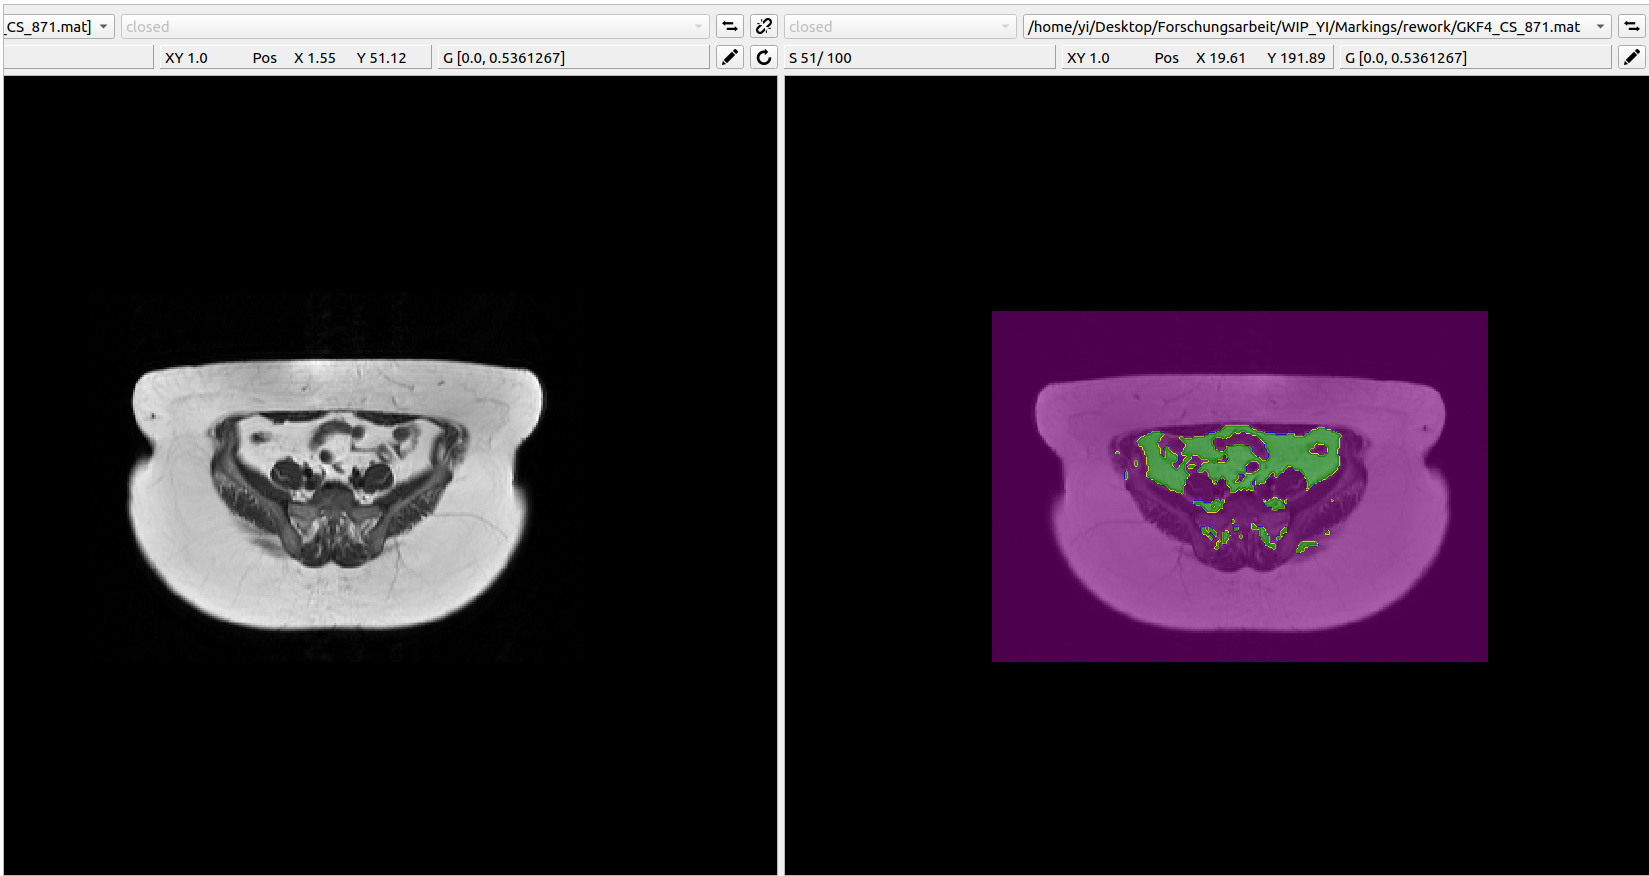
\includegraphics[width=\textwidth]{show_result.png}
		\caption[Show Result]{Show Result}
		\label{fig:show_result}
	\end{figure}
	\item Load previous
	\newline You can also load the previous images you have shown if you save it by triggering the corresponding item in menu \textit{File}.
\end{enumerate}

\subsection{Edit images}
There are several regular operations for having a better look at images.
\begin{enumerate}
	\item Set layout
	\newline If you want to view several images at the same time, you can click the button \textit{Set Layout}, then you can select how many grids you would like to show. When you click the first grid at the left top corner, it will remain/change to show one layout; If you select several continuous grids, the layout will be shown in the same way; But if you select any other single grid other than the first one, it will be ignored. 
	\begin{figure}[htbp]	
		\centering
		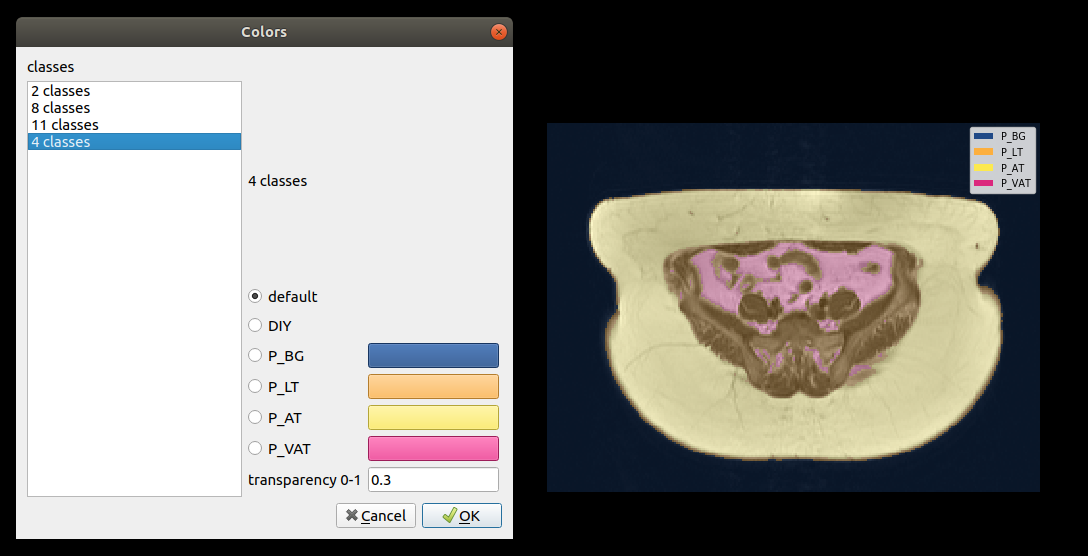
\includegraphics[width=\textwidth]{set_result_color.png}
		\caption[Set Result Color]{Set Result Color}
		\label{fig:set_result_color}
	\end{figure}
	\item Switch 2D/3D
	\newline If you want to have a look at a 3D image in three dimension at the same time, you can click the button \textit{2D/3D Switch}, then the layouts will be fixed as three columns with 2D images in XY, YZ and XZ individually, and you still can set layout rows.
	\item Rotate image
	\newline If the image is not shown in the right direction, you can click the button \textit{Flip Image} to rotate the current image 90$\degree$ in clockwise at each time. It is possible to rotate view in both 2D and 3D.
	\item Fit size
	\newline If the image is not shown in the right scale, you can click the button \textit{Fit image view} to change between automatic aspect or equalized aspect of axis scaling method. It is possible to fit size in both 2D and 3D.
	\item Rotate dimension
	\newline At the top right corner of each layout, there is a \textit{rotate} button to switch dimension from XY over YZ to ZX.
	\item Change slice
	\newline You can either scroll up/down mouse wheel or press up/down key to change slice.
	\item Change gray scale
	\newline You can move mouse and keep the wheel button pressed to change gray scale, or press right/left key can also realize the same goal. If you want to set the gray scale precisely, you can click the \textit{edit} button at the top right corner of each layout, and then type in the desired number in a pop up window and confirm it.
	\item Zoom/Move image
	\newline You can zoom in/out image ba pressing the right mouse button and move up/down. If the image is large scaled, you can also move the image by moving and pressing the left mouse button.
	\item Link on
	\newline If you want to move/zoom image in three dimension view, you can click the \textit{link} button. 
	\item Scroll 4D/5D image
	\newline If the image has four or five dimensions, you can move the fourth dimension forwards/backward by key \textit{1/2}, and move the fifth dimension forward/backward by key \textit{3/4}.
\end{enumerate}

\subsection{Edit result}
The flipping images and fitting size functions are not suitable for result images. 
\begin{enumerate}
	
	\item Set colors
	\newline The colors of mask(s) are initially set be default colors or the preferred colors saved in result file. If you want to edit the mask colors, you can trigger a color window by clicking the item in the menu \textit{Settings}. There are pre-defined 2, 8, and 11 classes supported, or the corresponding number of classes showing in the current result file. You can choose \textit{DIY} to set colors, hatches and transparency in the window and confirm it. In \textit{default} mode, the modification will not be saved. When you set the color for the last item in \textit{DIY} mode, you should at first check on the radio button in front of each color button, only then you can select the desired color for the corresponding class.
	\item Show class name
	\newline If there are more than one class in the result image, you can choose to show the name in the drop down box \textit{show class name}. Then the class name will be around cursor when you click left mouse button in the region. Additionally, there will be also a legend showing the names and colors of different classes at the left top corner. If the legend covers the image, you can click legend on/off to show the legend on/off.
	\item Set transparency
	You can either set transparency in the color window or on the slider bar \textit{Set transparency}. The contrast between images and masks will be changed.
\end{enumerate}

\subsection{Assistance}
There are also some assistant methods to have a deeper insight of image or to draw labels on the image more conveniently.
\begin{enumerate}
	\item Show information
	\newline If you want to view all local, global and built-in functions used in this GUI, you can click the button \textit{Show Information}. Then a window with a drop down box will pop up. And the selected item will be shown in a list in the window.	
	\item Cursor inspector
	\newline If you check on the cursor inspector, the cursor will be surrounded with two cross lines wherever you click left mouse button on the image. If the image is in three dimensional mode, the slices will be changed synchronously to the clicked cursor position.
	\begin{figure}[htbp]	
		\centering
		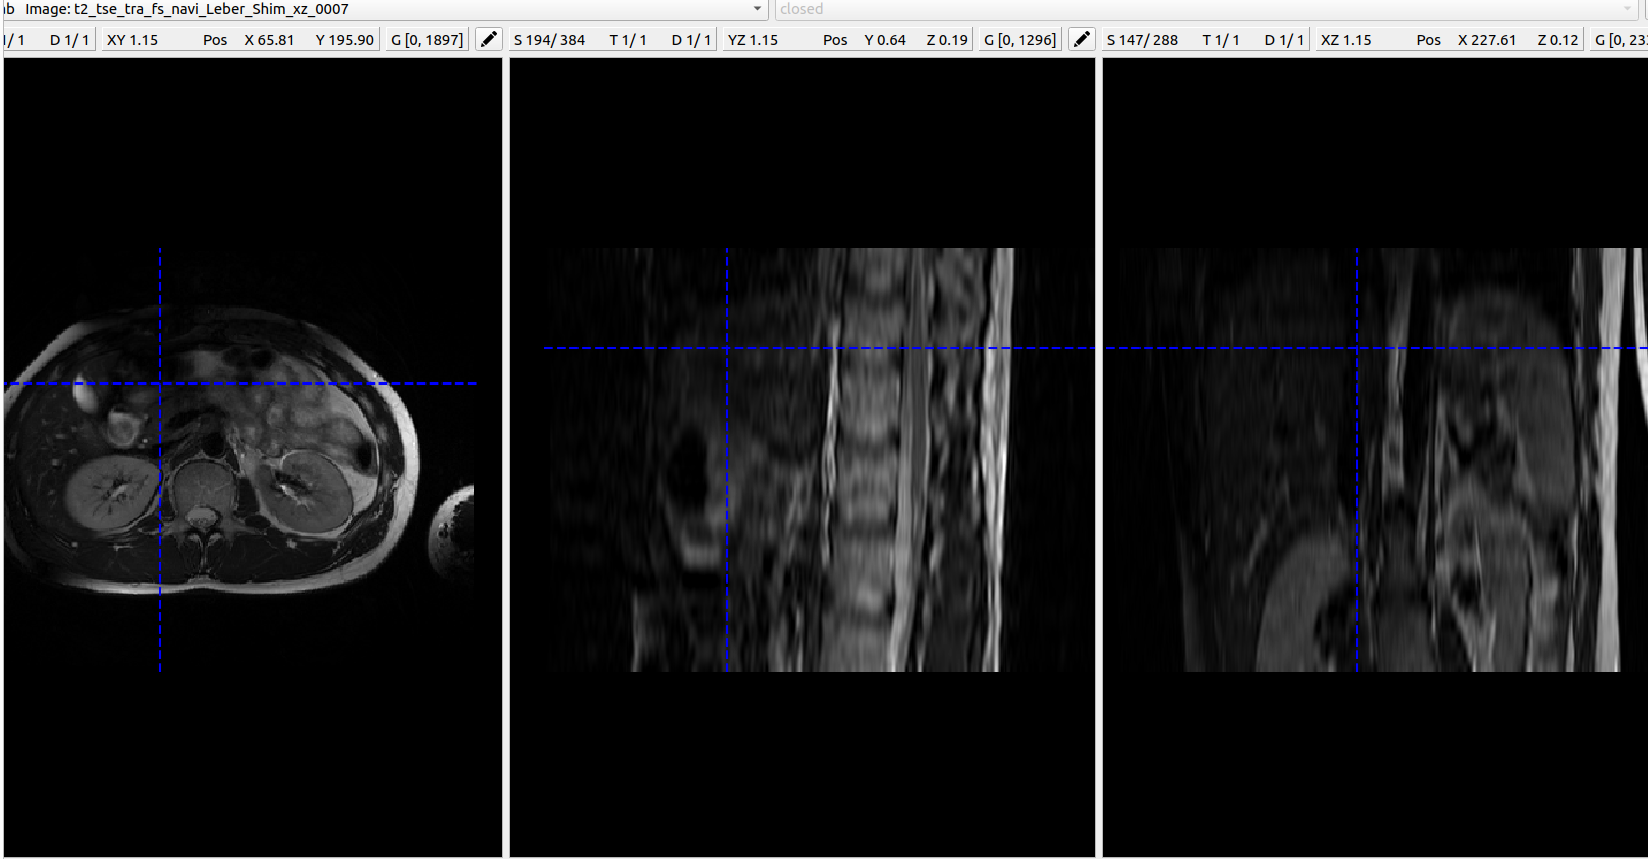
\includegraphics[width=\textwidth]{cursor_inspector.png}
		\caption[Cursor Inspector]{Cursor Inspector}
		\label{fig:cursor_inspector}
	\end{figure}
	\item Select region of interest(ROI)
	\newline Click the button \textit{ROI}, a independent window will pop up, showing the current image on the screen, you can select the \textit{ROI} under the image. And you can drag and change the size of a rectangular box to select ROI, and change the contrast and viewing the pixels of ROI.
	\begin{figure}[htbp]	
		\centering
		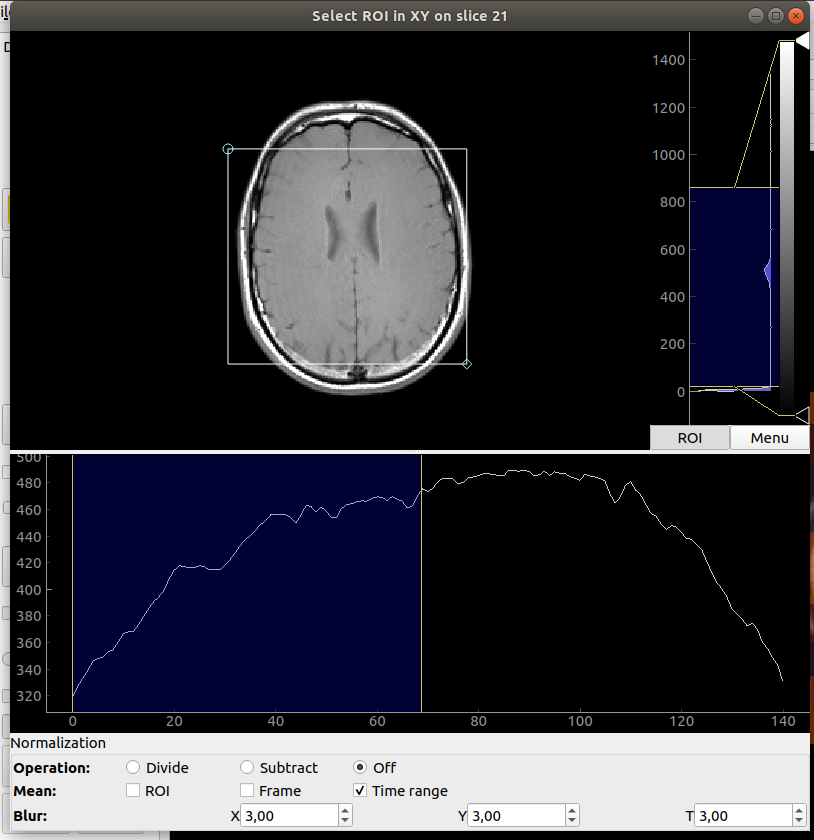
\includegraphics[width=\textwidth]{select_ROI.png}
		\caption[Select ROI]{Select ROI}
		\label{fig:select_ROI}
	\end{figure}
	
\end{enumerate}


\end{document}
